\documentclass{article}

\usepackage{fancyhdr}
\usepackage{extramarks}
\usepackage{amsmath}
\usepackage{amsthm}
\usepackage{amsfonts}
\usepackage{tikz}
\usepackage[plain]{algorithm}
\usepackage{algpseudocode}
\usepackage{enumerate}
\usepackage{braket}
\usepackage{color}
\usepackage{fontspec}
\usepackage{subfig}
\usepackage{booktabs}
\usepackage{multirow}

\usetikzlibrary{automata,positioning}

%
% Basic Document Settings
%

\topmargin=-0.45in
\evensidemargin=0in
\oddsidemargin=0in
\textwidth=6.5in
\textheight=9.0in
\headsep=0.25in

\linespread{1.1}

\pagestyle{fancy}
\lhead{\hmwkAuthorName}
\rhead{\hmwkClassNo: \hmwkTitle}
\cfoot{\thepage}

\renewcommand\headrulewidth{0.4pt}
\renewcommand\footrulewidth{0.4pt}

\setlength\parindent{0pt}

\newcommand{\hmwkTitle}{Homework Project\ \#3}
\newcommand{\hmwkDueDate}{April 6, 2023}
\newcommand{\hmwkClass}{Monte Carlo and Molecular Dynamics Simulation in Statistical Physics \& Materials Science}
\newcommand{\hmwkClassNo}{MSE504}
\newcommand{\hmwkClassInstructor}{Professor R. Car}
\newcommand{\hmwkAuthorName}{\textbf{Yihang Peng}}

%
% Title Page
%

\title{
    \vspace{2in}
    \textmd{\textbf{\hmwkClassNo\ -\ \hmwkClass:\ \hmwkTitle}}\\
    \normalsize\vspace{0.1in}\small{Due\ on\ \hmwkDueDate\ at 11:59 p.m.}\\
    \vspace{0.1in}\large{\textit{\hmwkClassInstructor}}
    \vspace{3in}
}

\author{\hmwkAuthorName}
\date{}

\newcommand{\pderiv}[2]{\frac{\partial #1}{\partial #2}}
\newcommand{\bpp}[3]{\left(\frac{\partial #1}{\partial #2}\right)_{#3}}
\newcommand{\dx}{\mathrm{d}x}
\newcommand{\E}{\mathrm{E}}
\newcommand{\Var}{\mathrm{Var}}
\newcommand{\Cov}{\mathrm{Cov}}
\newcommand{\Bias}{\mathrm{Bias}}
\newcommand{\diff}[1]{\mathrm{d} #1}
\newcommand{\e}[1]{\times 10^{#1}}
\newcommand{\Exp}[1]{\mathrm{e}^{#1}}
\newcommand{\mathpth}{\text{\pth}}
\newcommand{\inv}{^{-1}}
\newcommand{\ang}[1]{{\langle #1 \rangle}}

\setlength{\parskip}{1em}

\begin{document}

\maketitle

\pagebreak

\section{Simulation setup}

The molecular dynamics (MD) simulations are performed using LAMMPS package under periodic boundary conditions using the Verlet algorithm. I construct 5 simulation boxes of 108, 192, 256, 400, and 500 atoms interacting via a Lennard-Jones (LJ) potential. The LJ coefficients are set to $\epsilon = 0.0103$ eV, $\sigma = 3.405$ \AA, which are appropriate to Ar. The cut-off distance of the LJ potential is 15.0 \AA{} in my MD simulations. The mass of the particles is set to 39.948 u, which is the atomic mass of Ar. The time step of all simulations is 1 fs.

The initial configurations of particles are face-centered cubic (fcc) lattice, and I set the lattice parameter to 5.78015 \AA{} in order to achieve a constant density of 1.34 g/cm$^3$. Simulations with different numbers of atoms are achieved by changing the number of fcc unit cells in the simulation regions. I assign each atom a random velocity with Gaussian distribution corresponding to the temperature of 94 K, and run canonical (NVT) simulations at 94 K employing the Nose-Hoover thermostat in order to equilibrate the system in the liquid phase. I carefully monitor the output of the total energy of the system, and consider the simulation to have reached equilibrium when the energy converges to a constant value. The total time of canonical simulations is 100 ps. I store the position and velocity of all particles at each time step in a dump file with very high storage precision of \verb|%20.15g|.

For each cell size, I examine the output file (\verb|log.lammps|) of the canonical simulation and find a time step with a temperature close to 94 K. I use the particle configuration data of this time step in the dump file as the input for a 100 ps microcanonical (NVE) simulation test. I monitor the average temperature in the output file and only accepted this configuration data if the average temperature is between 93.5 K and 94.5 K, as shown in Table 1. This configuration becomes the input file for all subsequent microcanonical simulations for this cell size. Otherwise, I selected another time step from the canonical output file and repeat the above steps described in this paragraph. The reason for doing this is that diffusion coefficient is extremely sensitive to temperature according to the Arrhenius equation 
\begin{equation}
    D = D_0 \Exp{-\frac{\Delta H}{RT}}
\end{equation}
If there is a difference in temperature between simulations of different cell sizes, even if it's just a few Kelvin, the linearity of the data points in Fig. 4 will become terrible.

\begin{table}[!h]
    \centering
    \caption{The average temperature of the microcanonical simulation for different cell sizes.}
    \begin{tabular}{cc}
    \toprule
    Number of atoms & Average temperature (K) \\ \midrule
    108             & 94.25               \\
    192             & 93.65               \\
    256             & 94.33               \\
    400             & 93.98               \\
    500             & 94.36               \\ \bottomrule
    \end{tabular}
\end{table}

\section{The pair correlation function and the static structure factor}

\begin{figure}
    \centering
    \subfloat[$g(r)$]
    {
    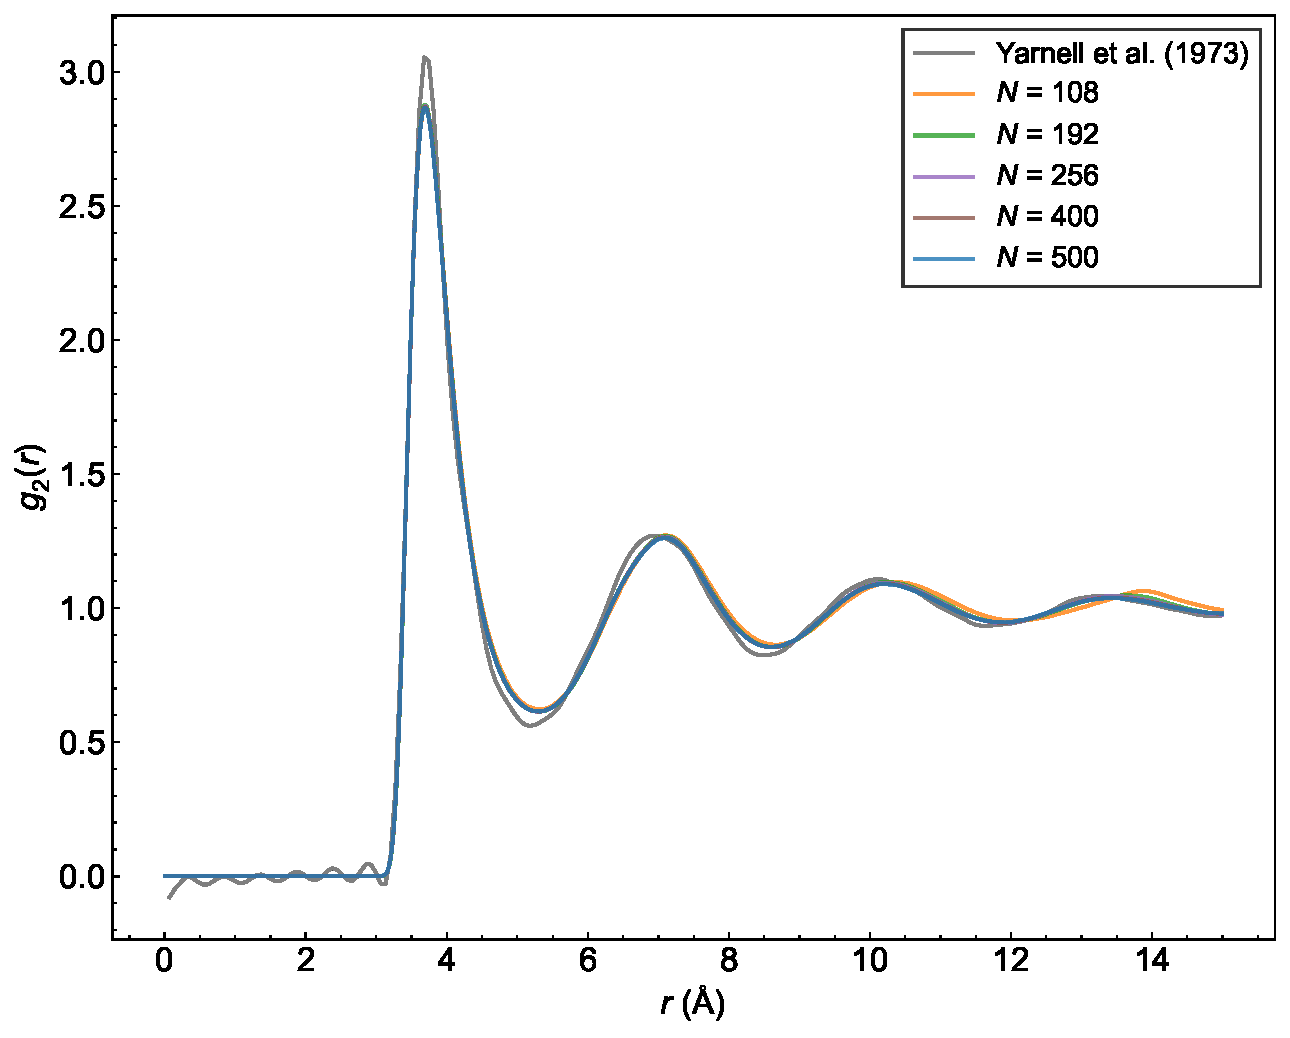
\includegraphics[width=0.75\textwidth]{./g2.pdf}
    }
    \\
    \subfloat[$S(q)$]
    {
    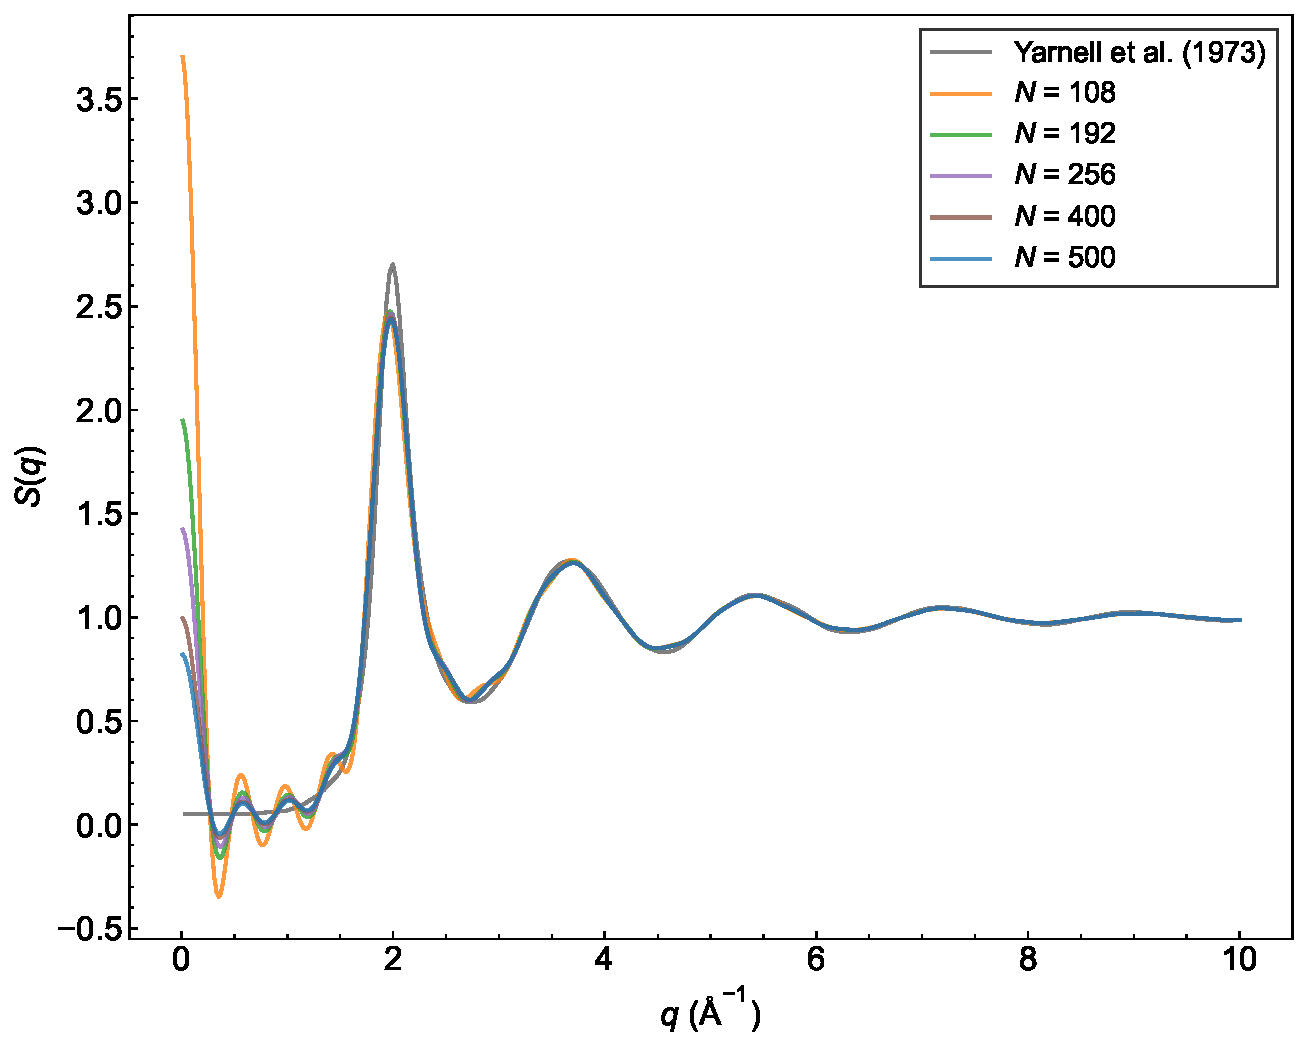
\includegraphics[width=0.75\textwidth]{./Sq.pdf}
    }
    \caption{The pair correlation function and the static structure factor of the LJ fluid.}
\end{figure}

The pair correlation function $g(r)$ can be calculated with \verb|compute ID group-ID rdf Nbin| in LAMMPS. I run microcanonical simulations for 5 ns and obtain the pair correlation function of the LJ fluid for 5 different cell sizes. My simulation results and the experimental results of Ar from J.L. Yarnell et al., {\it Phys. Rev}. A7, 2130 (1973) are shown in Fig. 1(a). The static structure factor $S(q)$ can be calculated using the Fourier transform technique
\begin{equation}
    S(q) = 1 + \rho \tilde{h}(q)
\end{equation}
where $\tilde{h}(q)$ is the Fourier transform of $h(r) = g(r) - 1$. The $S(q)$ results as well as the experimental data are plotted in Fig. 1(b). It should be noted that there may be some systematic errors due to the fact that the experimental results were measured at a temperature of 85 K, while my simulations were all conducted at 94 K. Overall, my simulation results are in good agreement with the experiment. It can be observed that as the size of the simulation cell increases, the computed $g(r)$ and $S(q)$ become more accurate and closer to the experimental results. This is particularly evident for larger values of $r$ in the $g(r)$ function, and smaller values of $q$ in the $S(q)$ function.

\section{The self-diffusion coefficient}

\begin{figure}
    \centering
    \subfloat[MSD]
    {
    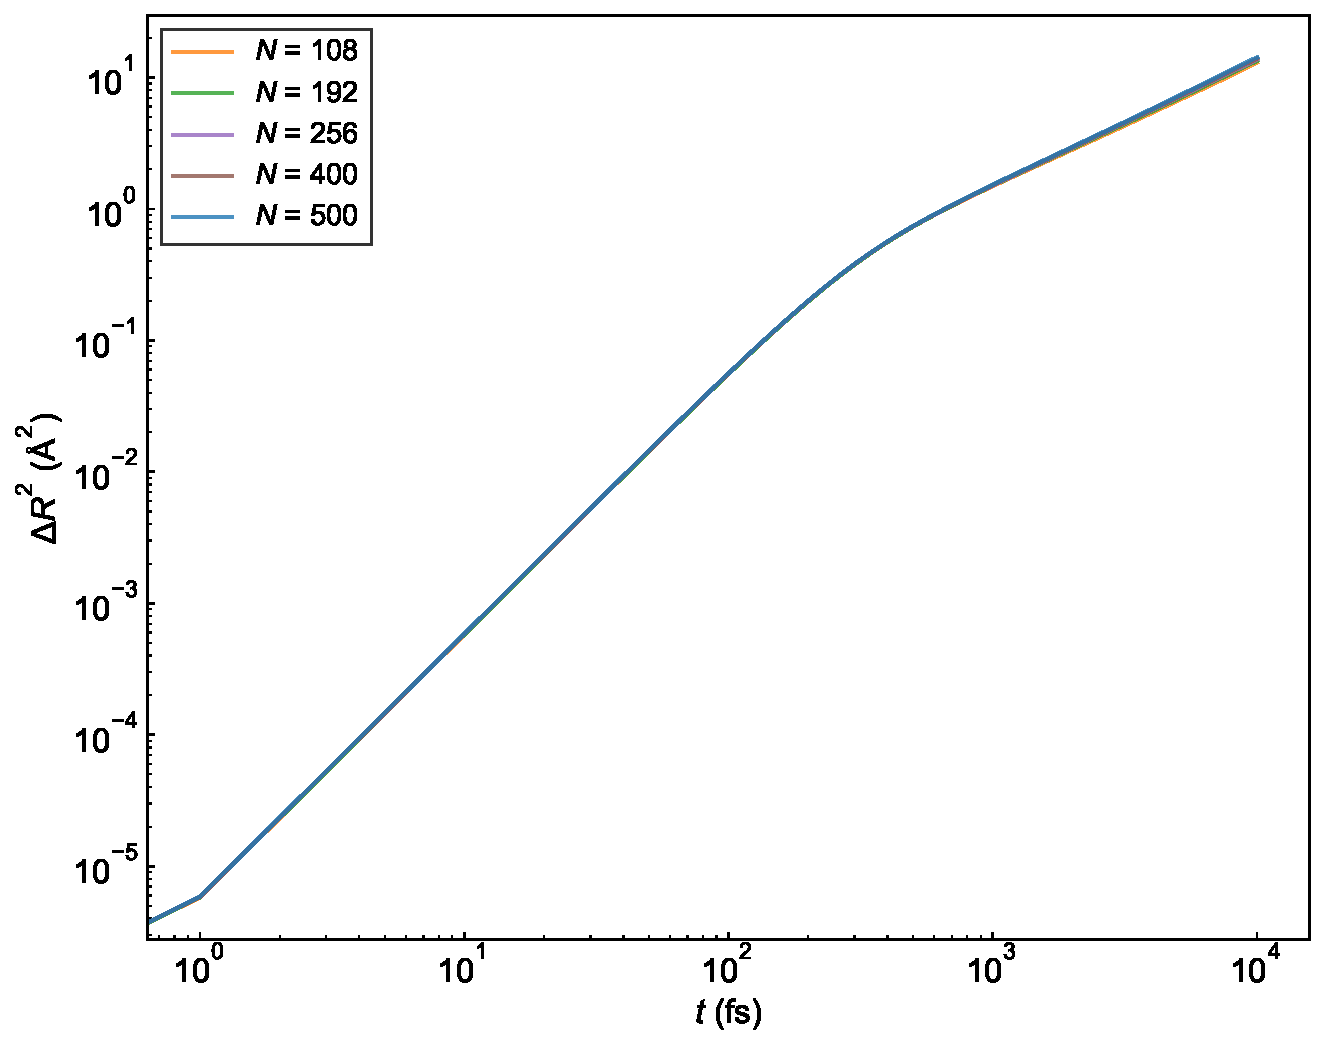
\includegraphics[width=0.75\textwidth]{./msd.pdf}
    }
    \\
    \subfloat[VACF]
    {
    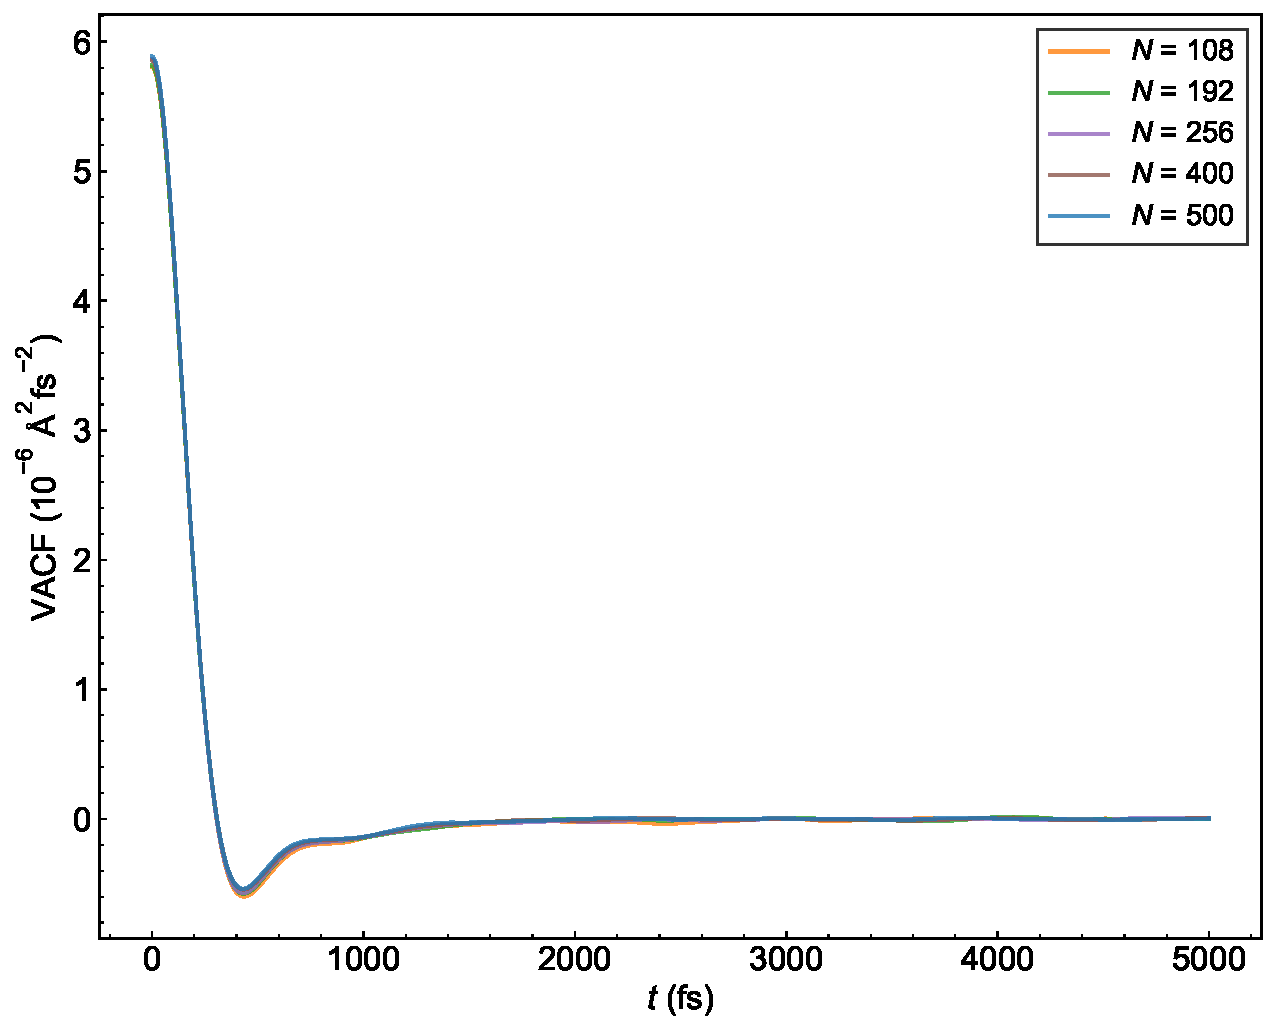
\includegraphics[width=0.75\textwidth]{./vacf.pdf}
    }
    \caption{The mean square displacement and velocity auto-correlation function of the LJ fluid.}
\end{figure}

According to Einstein relation, the self-diffusion coefficient, $D$, is the slope of mean square displacement (MSD, $\Delta R^2$)
\begin{equation}
    D = \lim _{t \rightarrow \infty} \frac{\Delta R^2}{6 t}=\lim _{t \rightarrow \infty} 
    \frac{\left \langle\left[\vec{r}\left(t+t_0\right)-\vec{r}\left(t_0\right)\right]^2\right \rangle}{6 t}
\end{equation}
where $\vec{r}(t)$ is the particle trajectories continuous in Cartesian space, and $\langle \cdots \rangle$ represents an average over all atoms. $\Delta R^2$ can be calculated with \verb|compute ID group-ID msd| in LAMMPS. $D$ can also be obtained using Kubo formula
\begin{equation}
    D = \frac{1}{3} \int_{0}^{\infty} C(t) \diff{t}
\end{equation}
where $C(t)$ is the velocity auto-correlation function $\ang{\mathbf{v}(t)\cdot \mathbf{v}(0)}$. velocity auto-correlation function (VACF) can be calculated with \verb|compute ID group-ID msd| in LAMMPS. I run microcanonical simulation for 10 ps and repeat the simulation for 1000 times for each cell size. Each repeated simulation starts from the last time step of the previous simulation, and the input file for the first simulation was described in Section 1.

The average results of MSD and VACF from 1000 simulations are shown in Fig. 2(a) and Fig. 2(b). According to Fig. 2(a), during the initial few hundreds of fs, MSD as a function of time resembles ballistic motion ($\Delta R^2 \propto t^2$), since particles haven't experienced the interactions. The diffusive motion ($\Delta R^2 \propto t$) is achieved at about $t \sim 10^3$ fs, and I only use the MSD after 2000 fs for linear fitting to calculate $D$. Similarly, to reduce the errors introduced by numerical integration when the VACF approaches zero, I only considered the first 5000 fs of VACF data when using the Kubo formula to calculate $D$. Fig. 2(b) shows that the VACF becomes negative at $t = 307$ fs and remains essentially negative as it goes to zero, which is known as the ``caging" effect. It is very different from the Langevin type of velocity auto-correlation ($\Exp{-k_B Tt / MD}$) for Brownian fluid. A more illuminating way of exhibiting this difference is to consider the power spectrum, which is Fourier transform of the VACF, given by
\[
    f(\omega) = \frac{k_B T}{MD} \int_{0}^{\infty} \frac{\ang{\mathbf{v}(t)\cdot \mathbf{v}(0)}}{\ang{\mathbf{v}^2}} \cos \omega t \diff{t} = \frac{1}{3D} \int_{0}^{\infty} C(t) \cos \omega t \diff{t}
\]
Fig. 3 shows $f(\omega)$ obtained from the VACF shown in Fig. 2(b). It has a broad maximum at about $\omega = 0.0035$ fs$^{-1}$, which is distinct from the Lorentzian $f(\omega) = \frac{a^2}{a^2 + \omega^2}$ for Brownian motion, also shown in Fig. 2(b).
\begin{figure}
    \centering
    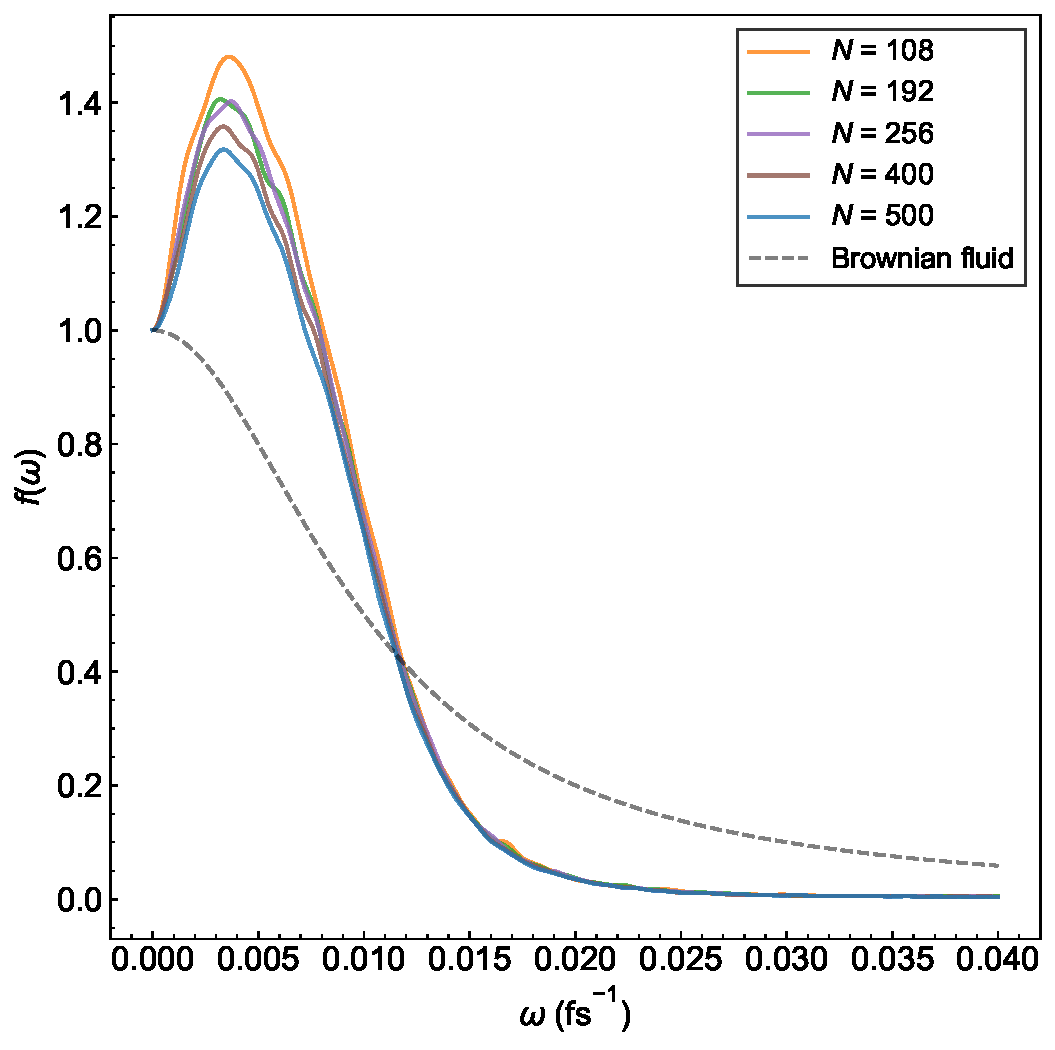
\includegraphics[width=0.7\textwidth]{ps.pdf}
    \caption{The power spectrum $f(\omega)$ of the velocity auto-correlation function. The Lorentzian spectrum of a Brownian fluid is also shown.}
\end{figure}

\begin{figure}
    \centering
    \subfloat[Einstein relation]
    {
    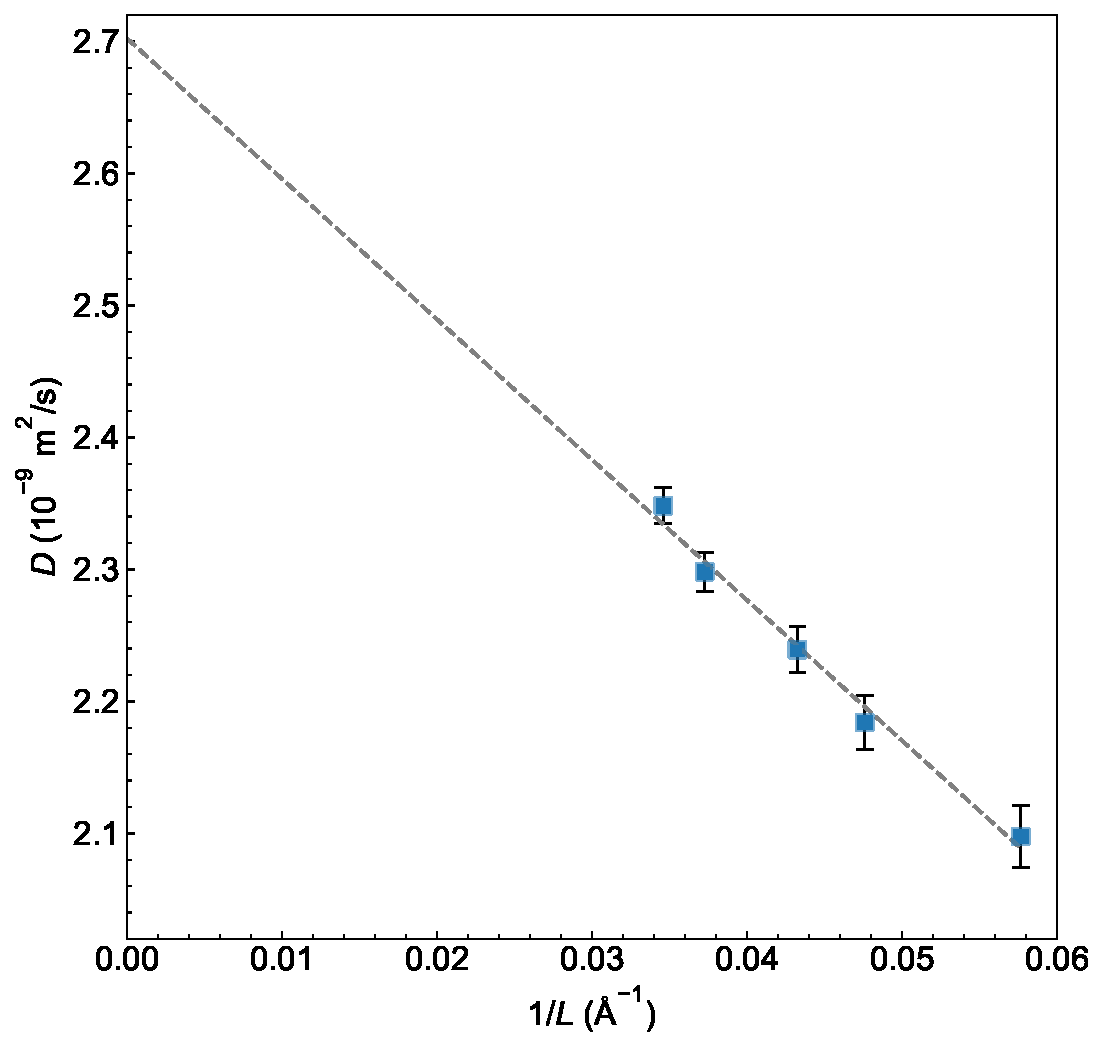
\includegraphics[width=0.65\textwidth]{D_msd.pdf}
    }
    \\
    \subfloat[Kubo formula]
    {
    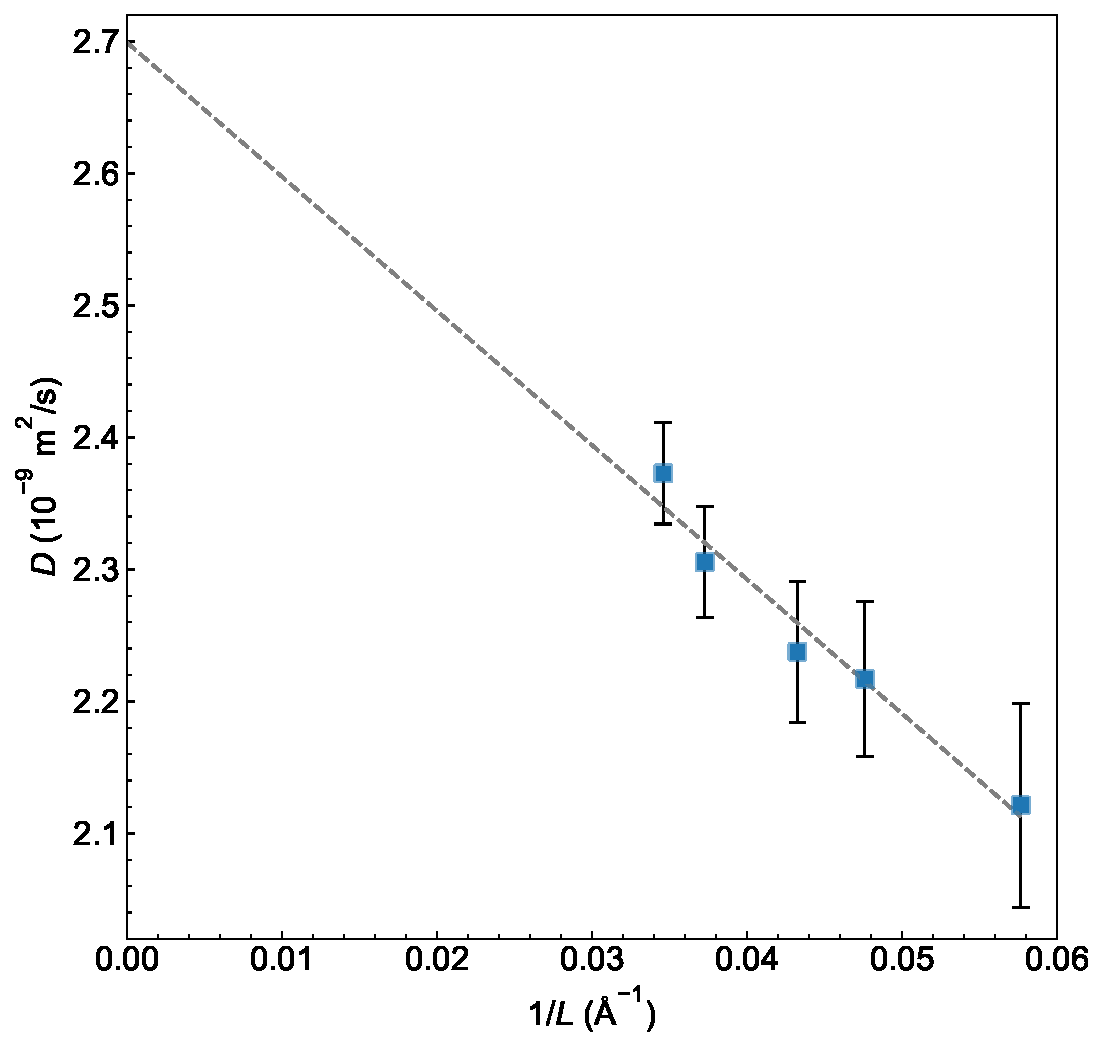
\includegraphics[width=0.65\textwidth]{D_vacf.pdf}
    }
    \caption{Diffusion coefficients of the LJ fluid for different cell sizes obtained from both Einstein relation and Kubo formula.}
\end{figure}
The calculated results of diffusion coefficients for different cell sizes are shown in Fig. 4.
The error bars are the 2SE of the 1000 simulation results for each data point. It is obvious that Einstein relation works better in this project, which shows much lower uncertainty than the Kubo formula. The size effect for $D$ can be found by writing out analytically the hydrodynamic limit given by
\begin{equation}
    D(L) = D_{\infty} - \frac{k_B T \zeta}{6 \pi \eta L}
\end{equation}
where $D_{\infty}$ is the thermodynamic limit of $D$ with infinite size, $\zeta$ is a numerical coefficient that is characteristic of the assumed periodic supercell, and $\eta$ is the translational shear viscosity. By fitting this extrapolation formula to the $D$ results, as shown in Fig. 4, I find that using Einstein relation, $D_{\infty} = 2.702 \times 10^{-9}\ \mathrm{m^2/s}$, $\eta = 183.9\ \mathrm{\mu Pa \cdot s}$. Similarly, using Kubo formula, $D_{\infty} = 2.699 \times 10^{-9}\ \mathrm{m^2/s}$, $\eta = 192.3\ \mathrm{\mu Pa \cdot s}$.

\begin{figure}[!t]
    \centering
    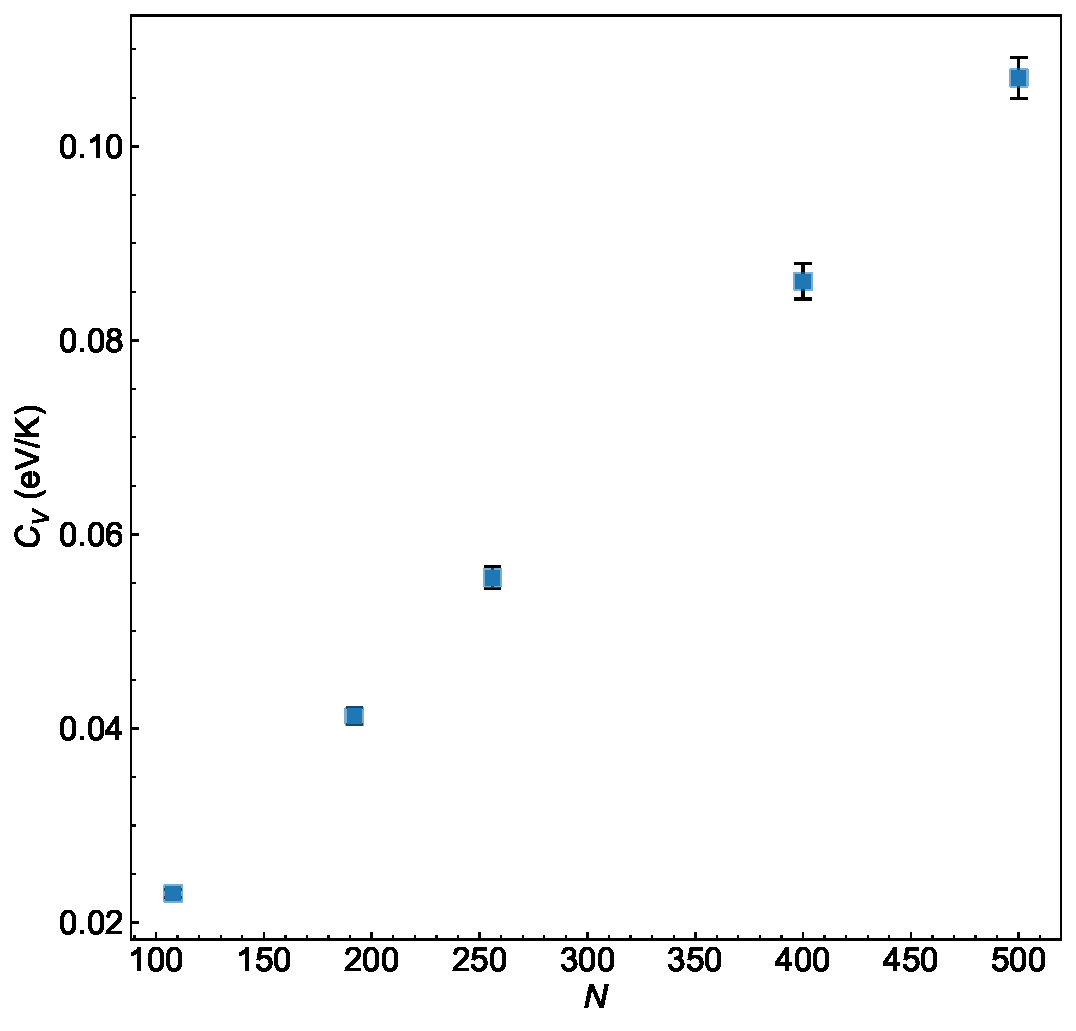
\includegraphics[width=0.6\textwidth]{Cv.pdf}
    \caption{The heat capacity of the LJ fluid.}
\end{figure}

\section{The heat capacity}

The heat capacity $C_V$ can be computed from the fluctuation of the kinetic energy $K$ of the particles, using the formula:
\begin{equation}
    \left \langle \delta K^2 \right \rangle_{N V E} = \frac{3 k_B^2 T^2 N}{2}\left(1-\frac{3 N k_B}{2 C_V}\right)
\end{equation}
where $\delta K \equiv K - \ang{K}$. I run microcanonical simulations for 1 ns and obtain the heat capacity of the LJ fluid for 5 different cell sizes, as shown in Fig. 5. The error bars are derived by splitting the 1-ns trajectory into 100 blocks and calculating 2SE of these 100 $C_V$ samples. The results show that the heat capacity is proportional to the number of atoms, and the uncertainty of $C_V$ increases with increasing cell size.


\end{document}
